\section{Samples}
\label{sec:samples}

All the MC samples used were processed centrally. 
As default for CMS, the signal samples use PDF4LHC15\_nlo\_mc\_pdfas set~\cite{Carrazza:2015hva, Butterworth:2015oua, Dulat:2015mca,Harland-Lang:2014zoa, Ball:2014uwa} in the four flavour scheme. The central value for the strong coupling is taken as $\alpha_s(m_Z) = 0.118$. %This analysis aims to investigate data collected by CMS in 2016, therefore, all the samples mentioned below have been produced in the 80X CMSSW releases. 
The samples used in this analysis have been processed by the standard CMS chain, including a detailed detector simulation with GEANT4. 
These samples have also been pre-processed by the central $\Hgg$ analysis framework FLASHgg, in order to obtain the most up-to-date photon energy, resolution and identification algorithms used by the $H\rightarrow\gamma\gamma$ analysis.

\subsection{Signal MC: resonant production}
%{\bf REALLY, we do not use the RS1 samples?}

To simulate the generic resonances we use {\tt MG5\_aMC@NLO}~\cite{Alwall:2014hca} at leading order. 
For the gluon fusion produced spin-2 resonance, we use the model for a KK-graviton in the bulk described in~\cite{Oliveira:2010uv}, which is an adaptation of the RS1 model of Ref.~\cite{aquino}, introducing  the relevant coupling modifications. 
The model files can be found in~\cite{WEDtwiki} and it is found to agree at the level of cross sections and branching ratios with the bulk WED scenario implemented by the authors of~\cite{Tuomas} in the {\tt CalcHep}~\cite{Belyaev:2012qa} framework. 
To simulate the scalar resonance, we use the Higgs Effective Model ~\cite{heft} that can found in the {\tt Feynrules} database~\cite{Alloul:2013bka}.
%We do not ask any additional jet with respect to the HH final state on the parton level simulation, so no matching is needed between matrix-element and parton shower.
%The radion fullSim signal samples, digitized with the Run-Dependent conditions {\bf CHECK this last}.

The spin-0 and spin-2 resonances are simulated with masses: 250, 260, 270, 280, 300, 320, 340, 350, 400, 450, 500, 550, 600, 650, 700,
750, 800, 900, 1000 \GeV, with 50k events each, assuming resonance width of 1 GeV. 
The cross sections for the interpretations can be found here~\cite{cx}. The {\tt MG5\_aMC@NLO} configuration cards used for the simulations are organized here~\cite{cards}. 
 
\subsection{Signal MC: nonresonant production}
\label{sec:nonresMC}
In the SM, Higgs boson pair production occurs predominantly by gluon-gluon fusion (GF) via an internal fermion loop. 
Since the Higgs boson couplings are defined by the particles masses, the top quark contribution is dominant, while couplings to light quarks are negligible \footnote{This assumption is motivated also in BSM theories where the Higgs sector is minimal (see also~\cite{Goertz:2014qia})}. 
%The extension of the latter feature as an assumption for BSM theories is well motivated if the Higgs sector is minimal (see also~\cite{Goertz:2014qia}).  
In the absence of new light states, the GF Higgs boson pair production at the LHC can then be generally described (to leading approximation) by five parameters controlling the tree-level interactions of the Higgs boson. 
%These five parameters, which will be discussed in detail in the following, are $\kappa_{\lambda}$, $\kappa_{t}$, $c_g$, $c_{2g}$, and $c_2$.
The Higgs boson trilinear coupling and the top Yukawa interaction exist in the SM Lagrangian, where the former is given by $\lambda_{SM}=m_h^2/2v^2$, with $v$ the vacuum-expectation value of the Higgs field. Deviations from SM values are parametrized with the multiplicative factors $\kappa_{\lambda}$ and $\kappa_{t}$, respectively. The contact interactions of the Higgs boson with gluons and those coupling two Higgs bosons with two gluons or a top-antitop quark pair, which could arise through the mediation of very heavy new states, are instead genuinely not predicted by the SM; they can be parametrized by the absolute couplings $c_g$, $c_{2g}$, and $c_2$. The relevant part of the Lagrangian then takes the form \par

\begin{eqnarray}
{\cal L}_h = 
\frac{1}{2} \partial_{\mu}\, h \partial^{\mu} h - \frac{1}{2} m_h^2 h^2 -
  {\kappa_{\lambda}}\,  \lambda_{SM} v\, h^3 
- \frac{ m_t}{v}(v+   {\kappa_t} \,   h  +  \frac{c_{2}}{v}   \, h\,  h ) \,( \bar{t_L}t_R + h.c.) \nonumber  \\ 
+ \frac{1}{4} \frac{\alpha_s}{3 \pi v} (   c_g \, h -  \frac{c_{2g}}{2 v} \, h\, h ) \,  G^{\mu \nu}G_{\mu\nu}\,.
\label{eq:lag}
\end{eqnarray}

The different Feynman diagrams contributing to a di-Higgs boson signal in {\em pp} collisions at leading order (LO) are shown in Fig.~\ref{fig:dia}.
The simulation setup used in this paper was produced by the authors of~\cite{Hespel:2014sla}. We use {\tt MG5\_aMC@NLO} as generator. The LO process is already at one-loop level; in the approach followed in~\cite{Hespel:2014sla}, loop factors are calculated on an event-by-event basis with a {\tt Fortran} routine on top of an $aMC@NLO$~\cite{Frixione:2010ra, Alwall:2014hca} effective model;

\begin{figure}[h]
\centering
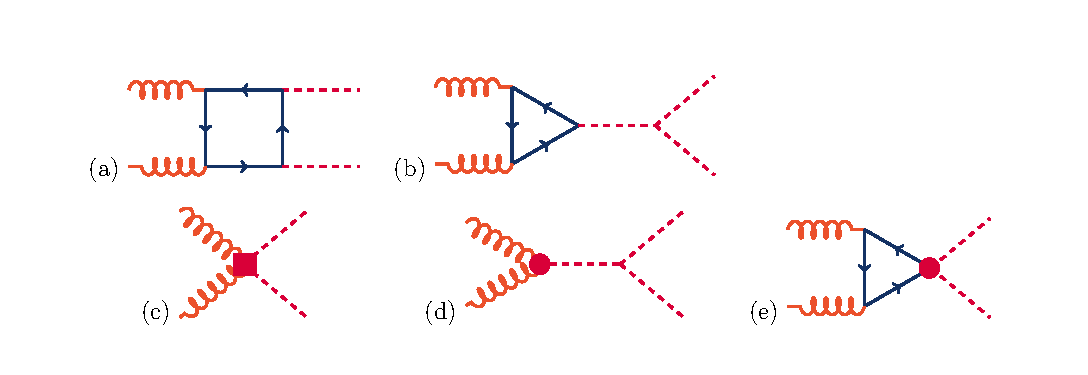
\includegraphics[scale=0.85]{figures/translation.pdf}
\caption{\small Feynman diagrams that contribute to Higgs boson pair production by gluon-gluon fusion at leading order. Diagrams (a) and (b) correspond to SM-like processes, while diagrams (c), (d), and (e) correspond to pure BSM effects: (c) and (d) describe contact interactions between the Higgs boson and gluons, and (e) exploits the contact interaction of two Higgs bosons with top quarks.   \label{fig:dia}}
\end{figure} 

In the Ref.~\cite{Dall'Osso:2015aia}, it was designed a method to partition the 5 dimensional parameter space in regions 
with similar LO kinematics. 
When the simulation was launched in the CMS system this work was in a preliminary version, we had simulated the samples 
using to the recommendations of the first version. The list of relevant parameters used in each sample is in Table~\ref{tab:bench}. 
 The {\tt MG5\_aMC@NLO} configuration cards used for the simulations are organized here~\cite{cards}. 
Since then, the metric used by the method was improved and the parameter space scan extended, resulting in a 
new set of benchmarks, that can be found in the last ArXiV version of the mentioned paper, and as well in~\cite{MelladoGarcia:2150771}.
The analytical formula that allows us to calculate cross sections for any point of the parameter space can be found in~\cite{CarvalhoAntunesDeOliveira:2130724}, and a handful script that calculates the cross sections point-by-point can be found in~\cite{hhrosetta}.  

\begin{table}
\centering
\small{
\begin{tabular}{|c||c|c|c|c|c|}
\hline
Node & $\kappa_{\lambda}$ & $\kappa_{t}$ & $c_2$ & $c_g$ & $c_{2g}$ \\\hline
1  &   1.0 & 1.0  &  0.0 &  0.0 &  0.0  \\ \hline
2  &   7.5 & 2.5  & -0.5 &  0.0    &  0.0      \\ \hline
3  &  15.0 & 1.5  & -3.0 & -0.0816 &  0.3010   \\\hline
4  &   5.0 & 2.25 &  3.0 &  0.0    &  0.0     \\\hline
5  &  10.0 & 1.5  & -1.0 & -0.0956 &  0.1240  \\ \hline
6  &   1.0 & 0.5  &  4.0 & -1.0    & -0.3780  \\ \hline
7  &   2.4 & 1.25 &  2.0 & -0.2560 & -0.1480  \\ \hline
8  &   7.5 & 2.0  &  0.5 &  0.0    &  0.0     \\ \hline
9  &  10.0 & 2.25 &  2.0 & -0.2130 & -0.0893  \\ \hline
10 &  15.0 & 0.5  &  1.0 & -0.0743 & -0.0668  \\ \hline
11 & -15.0 & 2.0  &  6.0 & -0.1680 & -0.5180  \\ \hline
12 &   2.4 & 2.25 &  2.0 & -0.0616 & -0.1200   \\ \hline
13 & -15.0 & 1.25 &  6.0 & -0.0467 & -0.5150   \\ \hline
\end{tabular}
}
\caption{\small Parameter values of the final benchmarks selected with $N_{clus} = 13$. 
The first cluster is the one that contains the SM sample. 
\label{tab:bench_old}}
\end{table} 

\subsubsection{Reweighting}
\label{sec:rewei}

We are considering a $2\to 2$ process at leading order. The two Higgs bosons are produced with identical transverse momenta ($p_{T}^{H}$), and they are back-to-back in azimuth at this order (before a parton shower). The final state can then be completely defined by three kinematic variables, if we ignore the irrelevant azimuthal angle of emission of the bosons. Furthermore, one of the three remaining variables can be used to isolate all the information related to the PDF of the colliding partons, which is also irrelevant to the physics of the production process once one focuses on a specific initial state (the gluon-gluon fusion process). The variable factorizing out the PDF modeling can be taken as the magnitude of the boost of the center-of-mass frame as seen in the laboratory frame. 

The two remaining variables, which provide direct information on the physics of GF HH production, can be chosen to be the invariant mass of the HH system ($m_{HH}$) and the modulus of the cosine of the  polar angle of one Higgs boson with respect to the beam axis ($|cos\theta^*|$). Since we are using parton-level information, this last variable is equivalent to the polar angle in the Collins-Soper frame ($|cos\theta^*_{CS}|$)~\cite{PhysRevD.16.2219}, which is commonly used in experimental analysis. The variables $m_{HH}$ and $|cos\theta^*|$ can thus be used to fully characterize the final state kinematics produced by different choices of the value of anomalous Higgs boson coupling parameters.

By construction the full-simulated samples listed in Tab.~\ref{tab:bench}  are good representatives of the kinematic space. 
Therefore, based in the generation level $m_{HH}$ and $|cos\theta^*|$, those can be used to construct 
samples to any other parameter space point. 

The procedure is made as follows: 
\begin{itemize}
\item For each new parameter space point we simulate $N$ events in {\tt MG5\_aMC@NLO};
\item We construct two dimensional histograms at generator-level of $m_{HH}$ and $cos\theta^*$, with 20$\GeV$-wide bins in the $m_{HH}$ and 0.2-wide bins in $cos\theta^*$ (without the moduli);
\item We construct the same histogram with the sum of all the full simulated samples described in the last section (signal dataset);
\item The new sample is constructed by weigthing the signal dataset event-by-event by:
 \begin{equation}
 W_{e} = \frac{New_{ij}}{D_{ij}}\,,
 \end{equation}
 where ($ij$) specify the bin in which the event $e$ belongs and $New_{ij}$ ($D_{ij}$) the number of events of the 
 new signal sample (signal dataset) in that bin. 
 \end{itemize}
 
 We produce reweighted samples for three types of theory scans. 
 First, a plain scan in $\kappa_{\lambda}$, while all the other parameters are kept as in SM ($\kappa_{t}$, $c_2 = c_g  = c_{2g} =0$), where the gen-level histograms are made from 50,000 events. 
 Then, a scan in the 2D plane defined by fixing  $c_2 = c_g  = c_{2g} =0$, with varying $\kappa_{\lambda}$ and $\kappa_{t}$. 

 \begin{table}[h]
\centering
\small{
\begin{tabular}{rccccc}
\hline
Benchmark & $\kappa_{\lambda}$ & $\kappa_{t}$ & $c_{2}$	& $c_{g}$ & $c_{2g}$ \\\hline
1 &	7.5	 & 1.0	 &	-1.0	& 0.0	& 0.0 \\
2 &	1.0	 & 1.0	 &	0.5		& -0.8	& 0.6 \\
3 &	1.0	 & 1.0	 &	-1.5	& 0.0	& -0.8 \\
4 &	-3.5 & 1.5  &	-3.0	& 0.0	& 0.0 \\
5 &	1.0	 & 1.0	 &	0.0		& 0.8	& -1 \\
6 &	2.4	 & 1.0	 &	0.0		& 0.2	& -0.2 \\
7 &	5.0	 & 1.0	 &	0.0		& 0.2	& -0.2 \\
8 &	15.0 & 1.0	 &	0.0		& -1	& 1 \\
9 &	1.0	 & 1.0	 &	1.0		& -0.6	& 0.6 \\
10 &	10.0 & 1.5   &	-1.0	& 0.0	& 0.0 \\
11 &	2.4	 & 1.0	 &	0.0		& 1		& -1 \\
12 &	15.0 & 1.0	 &	1.0		& 0.0	& 0.0 \\ \hline %cl no. 463
SM &	1.0 & 1.0	 &	0.0		& 0.0	& 0.0 \\
\hline
\end{tabular}
}
\caption{\small Parameter values of the twelve benchmarks and the Standard Model point.  \label{tab:bench}}
\end{table}
 
 \subsection{Background MC}

Even though the signal extraction and background modeling of this analysis are performed in a data-driven way, background simulated samples are used to validate the simulation of our signal description and to optimize the analysis. 
The main backgrounds for the $\bbgg$ final state come from either well-isolated photons coming from the hard scatter (prompt photons) or isolated photons reconstructed due to very collimated $\pi^{0}\to\gamma\gamma$ decays fragmented from jets (fake photons). 
These backgrounds are the same as the ones to the SM $\Hgg$ analysis.

We can classify these backgrounds with respect to the number of prompt and fake photons in the selected diphoton candidate. The prompt-prompt background events are simulated with the Sherpa generator; it includes the Born processes with up to 3 additional jets at LO accuracy as well as the box processes at LO. 
The prompt-fake and the fake-fake contributions are simulated with PYTHIA8, with a "Double-EM Enriched" filter\footnote{it requires a high $\pt$ and well isolated photon-like signal (electromagnetic activity) coming from photons, electrons, or neutral hadrons)} applied during production to improve the samples selection efficiencies. 
Additionally, a sample of Drell-Yan events decaying into electrons, simulated at NLO with {\tt MG5\_aMC@NLO}, is used, although its final contribution to the event yield is minimal due to the $M(\gamma\gamma) > 100 \gev$ selection cut.

\subsection{Data}

The data samples used in this analysis correspond to approximately $35.87$ fb$^{-1}$ of data collected in 2016.

